\documentclass[conference,compsoc, 10pt]{IEEEtran}

% *** CITATION PACKAGES ***
\ifCLASSOPTIONcompsoc
\usepackage[nocompress]{cite}
\else
\usepackage{cite}
\fi

\usepackage{graphicx}

\ifCLASSINFOpdf
\else
\fi
%papaya
\hyphenation{op-tical net-works semi-conduc-tor}
\newcommand{\Mod}[1]{\ (\mathrm{mod}\ #1)}
\linespread{1.5}

\begin{document}	

\title{RSA Algorithm\\ Algorithm Analysis}
\author{\IEEEauthorblockN{Geovanny Burgos Retana}
\IEEEauthorblockA{Computer Engineering Student\\
Instituto Tecnologico de Costa Rica\\
San Jose, Costa Rica\\
Email: geoburgosretana@gmail.com}
\and
\IEEEauthorblockN{Anthony Leandro}
\IEEEauthorblockA{Computer Science Student\\
Instituto Tecnologico de Costa Rica\\
Limon, Costa Rica\\
Email: Anthonylle@hotmail.com}
\and
\IEEEauthorblockN{Bryan Mena Villalobos}
\IEEEauthorblockA{Computer Engineering Student\\
Instituto Tecnologico de Costa Rica\\
Heredia, Costa Rica\\
Email: mena97villalobos@gmail.com}}


\maketitle
\large
\begin{abstract}
	\large
	The abstract goes here.
\end{abstract}

\IEEEpeerreviewmaketitle


\section{Introduction}
RSA algorithm, first published on 1977 by Ron Rivest, Adi Shamir, and Len Adleman,  is a public-key cryptosystem, in this days, often used in various web servers, browsers and commercial system to protect web traffic among some other things like email encryption. In this type of cryptosystem the encryption key and the decryption key are different also, the encryption is public while de decryption key is private. This cryptosystem is base on the difficulty of factoring to prime large numbers.

\section[12pt]{Introduction}

RSA algorithm, first published on 1977 by Ron Rivest, Adi Shamir, and Len Adleman,  is a public-key cryptosystem, in this days, often used in various web servers, browsers and commercial system to protect web traffic among some other things like email encryption In this type of cryptosystem the encryption key and the decryption key are different also, the encryption is public while de decryption key is private. This cryptosystem is base on the difficulty of factoring to prime large numbers.

\section{The Algorithm}
Taking the words of Weisstein, E. RSA encryption is defined as "A public-key algorithm which uses prime factorization as the trapdoor one-way function". Given the formula $(m^e)^d \equiv m (mod n)$ the principle behind RSA is that is easy to find $e, d, n$ such as the formula is true, but is very difficult even impossible, finding $d$, even knowing $m, e, n$. As mention before RSA consists of a public key and a private key, public key is used to encrypt and private key is used to decrypt the message in a reasonable time, from the formula given before, public key is represented by the integers $e$ and $n$, and, the private key, is represented by d this led us with $m$, $m$ represents the message to encrypt

\subsection{How RSA works?}
First of all, we imagine that two individuals wants to exchange an encrypted message with RSA, $P_{1}$ has a public and a private key, $P_{1}$ shares the public key with $P_{2}$ when $P_{2}$ has the key he proceed to encrypt the message and send it to $P_{1}$, is important to clarify that only $P_{1}$ has the private key wich is used to decrypt the message, encryption and decryption process are describe below.  
\subsubsection{Encryption}
In encryption process the first step to follow is to turn M (message to send) into an integer m, such that 0 ≤ m < n in this step RSA uses a protocol such as the integer m will not felt into a range of integers that isn't secure. After this computing c (encrypted message) will be easy, using Alice's public key e as the following:
$c \equiv m^e \Mod{n}$
\subsubsection{Decryption}
Decryption is as easy as to use the private key $d$ in the following way:\newline
$c^d \equiv (m^e)^d \equiv m \Mod{n}$\newline
This way the message is recovered with the private key

\subsection{Before RSA}
RSA, in a certain way, was the first implementation of public key encryption, but, as seen in \textbf{\textit{The history of Non-Secret Encryption}} by J.H. Ellis public key encryption was long before been developed, in 1970 J. H. Ellis conceive a non-secret digital encryption(today known as public key encryption), in this time Ellis couldn't see a way to implement this type of encryption but in 1973 an employee of GCHQ came with the basic idea of RSA encryption base on Ellis work, but, as the new techniques discover on GCHQ that are potentially harmful, by definition, are classified information, this implementation was kept on secret.

\subsection{Actual panorama}
With the breakthrough in quantum computers is known that Shor's algorithm broke a 768-bit key (usually key sizes variate from 1024 to 4096 bits), this give us an idea of how quantum computers may change our way of thinking and what a breakout it would be since almost every of our actual encryption methods are base on prime number's difficulty to be generated

\section{Random and Pseudo-random number generation}
As the title says there are different ways to find a random number, knowing that the idea of RSA is to keep secure data via public and private keys, RSA needs a complex algorithm that not only generates this keys as a random number, but also needs to be an algorithm that generates random numbers in a secure way, keeping away  things like repeated random numbers or a pattern to generate them. The to basic ways to find random numbers are pseudo-random generation and random generation, as mention before random number generation must be unpredictable but in the case of pseudo random generation knowing the seed used to generate this numbers makes easy to predict the next pseudo random number generated, so as we can see  pseudo random generation is not feasible if we want a completely secure method to encrypt, next we have random generation, in random generation a non deterministic algorithm is used, as said before the number generated must be unpredictable so in random numbers generation may inputs, like keystrokes or mouse movements, may be used to ensure the randomness of the number generated. As seen in sections below this paper is base on the use of pseudo random numbers generation because the use of random generation as said in \textit{A Statistical Test Suite for Random and Pseudorandom Number Generators for Cryptographic Applications} (2010) "... may still be deficient when evaluated by statistical tests. In addition, the production of high-quality random numbers may be too time consuming, making such production undesirable when a
large quantity of random numbers is needed"(p.1-2)\newline
Also the use of pseudo random generation may be a better way to get out with this problems base on the quote of \textit{A Statistical Test Suite for Random and Pseudorandom Number Generators for Cryptographic Applications}
\begin{center}
	Ironically, pseudorandom numbers often appear to be more random than random numbers obtained from
	physical sources. If a pseudorandom sequence is properly constructed, each value in the sequence is
	produced from the previous value via transformations that appear to introduce additional randomness. A
	series of such transformations can eliminate statistical auto-correlations between input and output. Thus,
	the outputs of a PRNG may have better statistical properties and be produced faster than an RNG. (p.1-2)
\end{center}
\section{Methodology}
This section show how RSA can be analyzed by its complexity in order to classify the algorithm in a set of methods with different usages but with the same Big O order and how the experiments will proceed towards gather information about its behavior when it has different encryption and decryption requests.

\subsection{RSA Complexity Analysis}


\subsection{List of Experiments}
For the following experiments, there will be some tests to do in order to get detailed results. Those experiments are:



\begin{itemize}
	\item Encrypt and Decrypt a short word with at least 10 characters.
	\item Encrypt and Decrypt the lyric of Pendulum - Self vs Self song in a single line string.
	\item Use pseudo random number generator to get the prime numbers in a key.
	\item Use truly random number generator to get the prime numbers in a key.
\end{itemize}


\section{Experiments}
The time it takes for a laptop (Processor: Intel Dual-Core i3-4005U 1.70GHz) to show some tests mentioned in the methodology and other tests to get a better result is shown in the following graph, on the y axis is measured running Milliseconds for each test string with the number of letters per string that is displayed on the x-axis.

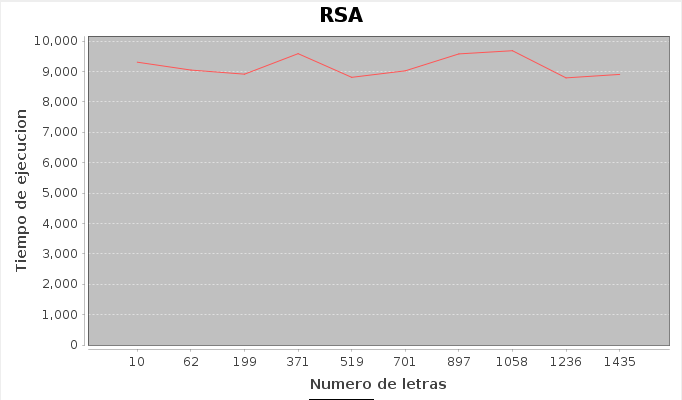
\includegraphics[scale=0.3]{Rsa_definitivo.png}
	
\section{Analysis and Results}
The results obtained in the graph shown in the previous section of experiments show that the number of characters that have the string entered in the program of the algorithm RSA does not have great importance in the case of encrypting or deciphering a word or a text. The algorithm takes a longer time in the random generation and generation of the integer that supports the large number that is generated at the time of encrypting the string.\newline
It was also observed that in order to encrypt for each letter that was in the chain the size of BigInteger should at least quadruple the size of the chain. That is to say that for a string of eight characters the size of the BigInteger must be at least 32.\newline
In the document has a section of randoms that explains that it is a random and a pseudo-random, it should be mentioned that it is not taken into account in these last two sections due to problems with the implementation, but as randomized investigations are the best Way to cry As is true at random, which implies a better efficiency at the moment of crying.

\section{Conclusion}
The conclusion goes here.

\large
\begin{thebibliography}{1}
\bibitem{IEEEhowto:kopka}
Boneh, D (November, 1998). Twenty Years of Attacks on the RSA Cryptosystem, Retrieve from: http://crypto.stanford.edu/~dabo/pubs/papers/RSA-survey.pdf

\bibitem{IEEEhowto:kopta}
Ellis, J.H. (January, 1970). The possibility of secure non-secret analogue encryption, Retrieve from: http://cryptocellar.org/cesg/possnse.pdf

\bibitem{IEEEhowto:kopta}
Ellis, J.H. (May, 1970). The possibility of secure non-secret analogue encryption, Retrieve from: https://www.gchq.gov.uk/file/cesgresearchreportno3007pdf-2

\bibitem{IEEEhowto:koopta}
Ellis, J.H. 1987. The History of Non-Secret Encryption. Retrieve from: https://web.archive.org/web/20130404174201/\newline
https://cryptocellar.web.cern.ch/cryptocellar/cesg/ellis.pdf

\bibitem{IEEEhowto:kopka}
Weisstein, Eric W. "RSA Encryption." From MathWorld--A Wolfram Web Resource. Retrieve from: http://mathworld.wolfram.com/RSAEncryption.html

\bibitem{IEEEhowto:kopka}
R.L.Rivest, A.Sharmir, L.Adleman: A method for obtaining digital signatures and public key Cryptosystems”, Tata McGraw-Hill Retrieve from: http://people.csail.mit.edu/rivest/Rsapaper.pdf

\bibitem{IEEEhowto:kopta}
Williamson, Malcolm J. (January 21, 1974). Non—secret encryption using a finite field. Retrieve from:
https://www.gchq.gov.uk/sites/default/files/document\_files/\newline nonsecret\_encryption\_finite\_field\_0.pdf

\end{thebibliography}

\end{document}


